\section{Results \& Discussion}
\label{sec:results}

The stability radius methodology was applied to the set of $N=31$ candidates. Rather than producing a single optimal schedule, the analysis reveals a landscape of solutions whose robustness depends on the interplay between strategic priorities (criteria importance vector) and decision-maker attitude (orness). In the current unified grid formulation, this yields an LP weight-space dimension of $K=24$ for the Baseline scenario and $K=30$ for the Sustainability scenario. Across the tested configurations, three distinct alternatives emerged as robust choices: \textbf{T1\_D300\_S33}, \textbf{T3\_D300\_S33}, and \textbf{T3\_D500\_S42}.

\subsection{Robustness Analysis}

The stability results for both the Baseline and Sustainability scenarios are summarized in Table~\ref{tab:combined_stability}. The magnitude of $\rho$ serves as a confidence index: larger values indicate that the selected alternative remains optimal under a wider range of admissible weight perturbations.

\begin{table}[htbp]
\centering
\caption{Most robust alternatives and stability radii ($\rho$) across scenarios and attitudinal profiles. The \textit{Second most stable} column indicates the alternative with the second-largest stability radius, highlighting close competitors.}
\label{tab:combined_stability}
\resizebox{\textwidth}{!}{
\begin{tabular}{llccclc}
\toprule
\textbf{Scenario} & \textbf{Profile} & \textbf{Most Robust} & \textbf{$\rho$} & \textbf{Opt. Orness} & \textbf{Second Most Stable} & \textbf{$\rho_{2nd}$} \\
\midrule
\multirow{4}{*}{\textbf{Baseline}}
 & Risk-Averse & \textbf{T1\_D300\_S33} & 0.0265 & 0.311 & T3\_D300\_S33 & 0.0173 \\
 & Neutral & \textbf{T3\_D300\_S33} & 0.0387 & 0.498 & T1\_D300\_S33 & 0.0358 \\
 & Optimistic & \textbf{T3\_D300\_S33} & 0.0248 & 0.687 & T1\_D300\_S33 & 0.0236 \\
 & Full-Spectrum & \textbf{T3\_D300\_S33} & 0.0387 & 0.498 & T1\_D300\_S33 & 0.0358 \\
\midrule
\multirow{4}{*}{\textbf{Sustainability}}
 & Risk-Averse & \textbf{T3\_D500\_S42} & 0.0214 & 0.315 & T1\_D300\_S33 & 0.0175 \\
 & Neutral & \textbf{T3\_D500\_S42} & 0.0320 & 0.482 & T1\_D300\_S33 & 0.0306 \\
 & Optimistic & \textbf{T1\_D300\_S33} & 0.0199 & 0.683 & T3\_D500\_S42 & 0.0197 \\
 & Full-Spectrum & \textbf{T3\_D500\_S42} & 0.0320 & 0.482 & T1\_D300\_S33 & 0.0306 \\
\bottomrule
\end{tabular}
}
\end{table}

A notable finding is that the \textit{Risk-Averse} selection is itself scenario dependent. Under the Baseline scenario, the most robust alternative is \textbf{T1\_D300\_S33}, reflecting the dominance of its technical margins when operational priorities remain primary. Under the Sustainability scenario, the most robust alternative becomes \textbf{T3\_D500\_S42}, indicating that a conservative attitudinal profile does not necessarily imply a purely technical choice once environmental and social criteria receive substantial importance mass.

As attitudes shift towards neutrality and optimism, the decision boundary moves differently across scenarios. In the Baseline scenario, the most robust alternative becomes \textbf{T3\_D300\_S33} for both the \textit{Neutral} and \textit{Optimistic} intervals. In the Sustainability scenario, \textbf{T3\_D500\_S42} remains dominant for \textit{Risk-Averse} and \textit{Neutral} attitudes, but the most robust choice shifts to \textbf{T1\_D300\_S33} in the \textit{Optimistic} interval. This pattern supports the conclusion that the most stable solution depends jointly on the strategic importance vector and on the degree of compensation admitted by the decision-maker.

In almost all configurations, the second most stable alternative is one of the other two robust candidates. For instance, in the Baseline/\textit{Neutral} case, the gap between the most robust alternative (\textbf{T3\_D300\_S33}, $\rho \approx 0.0387$) and the second most stable (\textbf{T1\_D300\_S33}, $\rho \approx 0.0358$) is small. The same occurs in the Sustainability/\textit{Optimistic} case, where \textbf{T1\_D300\_S33} and \textbf{T3\_D500\_S42} are separated by less than $2 \times 10^{-4}$ in stability radius. These narrow gaps indicate contested regions where the decision remains sensitive to minor preference adjustments. By contrast, the Baseline/\textit{Risk-Averse} case presents a clearer selection.

Notably, alternatives like \textbf{T3\_D900\_S73} and \textbf{T5\_D500\_S42} appear sporadically with small positive radii ($\rho < 0.02$). While these are mathematically non-dominated for some weight values, their lack of a substantial stability region makes them practically irrelevant for robust decision-making compared to the other three identified above.

It is instructive to compare these robustness-driven selections with the original competition rankings (Table~\ref{tab:solver_results}). The ROADEF/EURO Challenge scoring function, a weighted sum of mean risk and excess, naturally improves with longer computation times as solvers refine their solutions: the best competition score in the solution pool is attained by \textbf{T1\_D900\_S42} with 47\,508.29. However, none of these top-scoring alternatives emerge as robustly optimal in the multi-criteria analysis. The discrepancy arises because the competition metric collapses multiple dimensions into a single scalar, masking trade-offs that matter in practice. The proposed framework, by contrast, preserves the full criterion structure and explicitly accounts for decision-maker attitudes. Notably, the three robust alternatives identified here, \textbf{T1\_D300\_S33} (47\,736.27), \textbf{T3\_D300\_S33} (47\,684.20), and \textbf{T3\_D500\_S42} (47\,694.37), become dominant once robustness to weight uncertainty and attitudinal profiles is considered. This highlights a key insight: optimizing a competition score does not guarantee a robust operational decision when stakeholder priorities or aggregation preferences may vary.

The physical rationale behind these selections can be understood by examining the normalized performance of each alternative (Table~\ref{tab:dm_matrix} and Figure~\ref{fig:radar_chart}). \textbf{T1\_D300\_S33} achieves the maximum values in \textit{Reliability Stress} and \textit{Robustness Slack}, and it also attains a near-maximum value in \textit{Risk Volatility} (0.991). This technical strength explains its persistence whenever reliability remains a prerequisite. Its main relative weakness is \textit{Summer Eco-Stress} (0.799), which limits its stability once sustainability criteria and compensatory attitudes become more influential. \textbf{T3\_D500\_S42} combines the maximum values in \textit{Robustness Slack} and \textit{Summer Eco-Stress} with strong scores in the remaining criteria, which explains why it dominates the Sustainability scenario under \textit{Risk-Averse} and \textit{Neutral} attitudes. \textbf{T3\_D300\_S33} provides the strongest \textit{Max Critical Overlap} score (0.968), together with the maximum \textit{Social Weekend Risk} value and a perfect \textit{Robustness Slack} score. This profile explains its emergence as the most robust alternative in the Baseline scenario once some degree of compensation is admitted.

\begin{figure}[htbp]
    \centering
    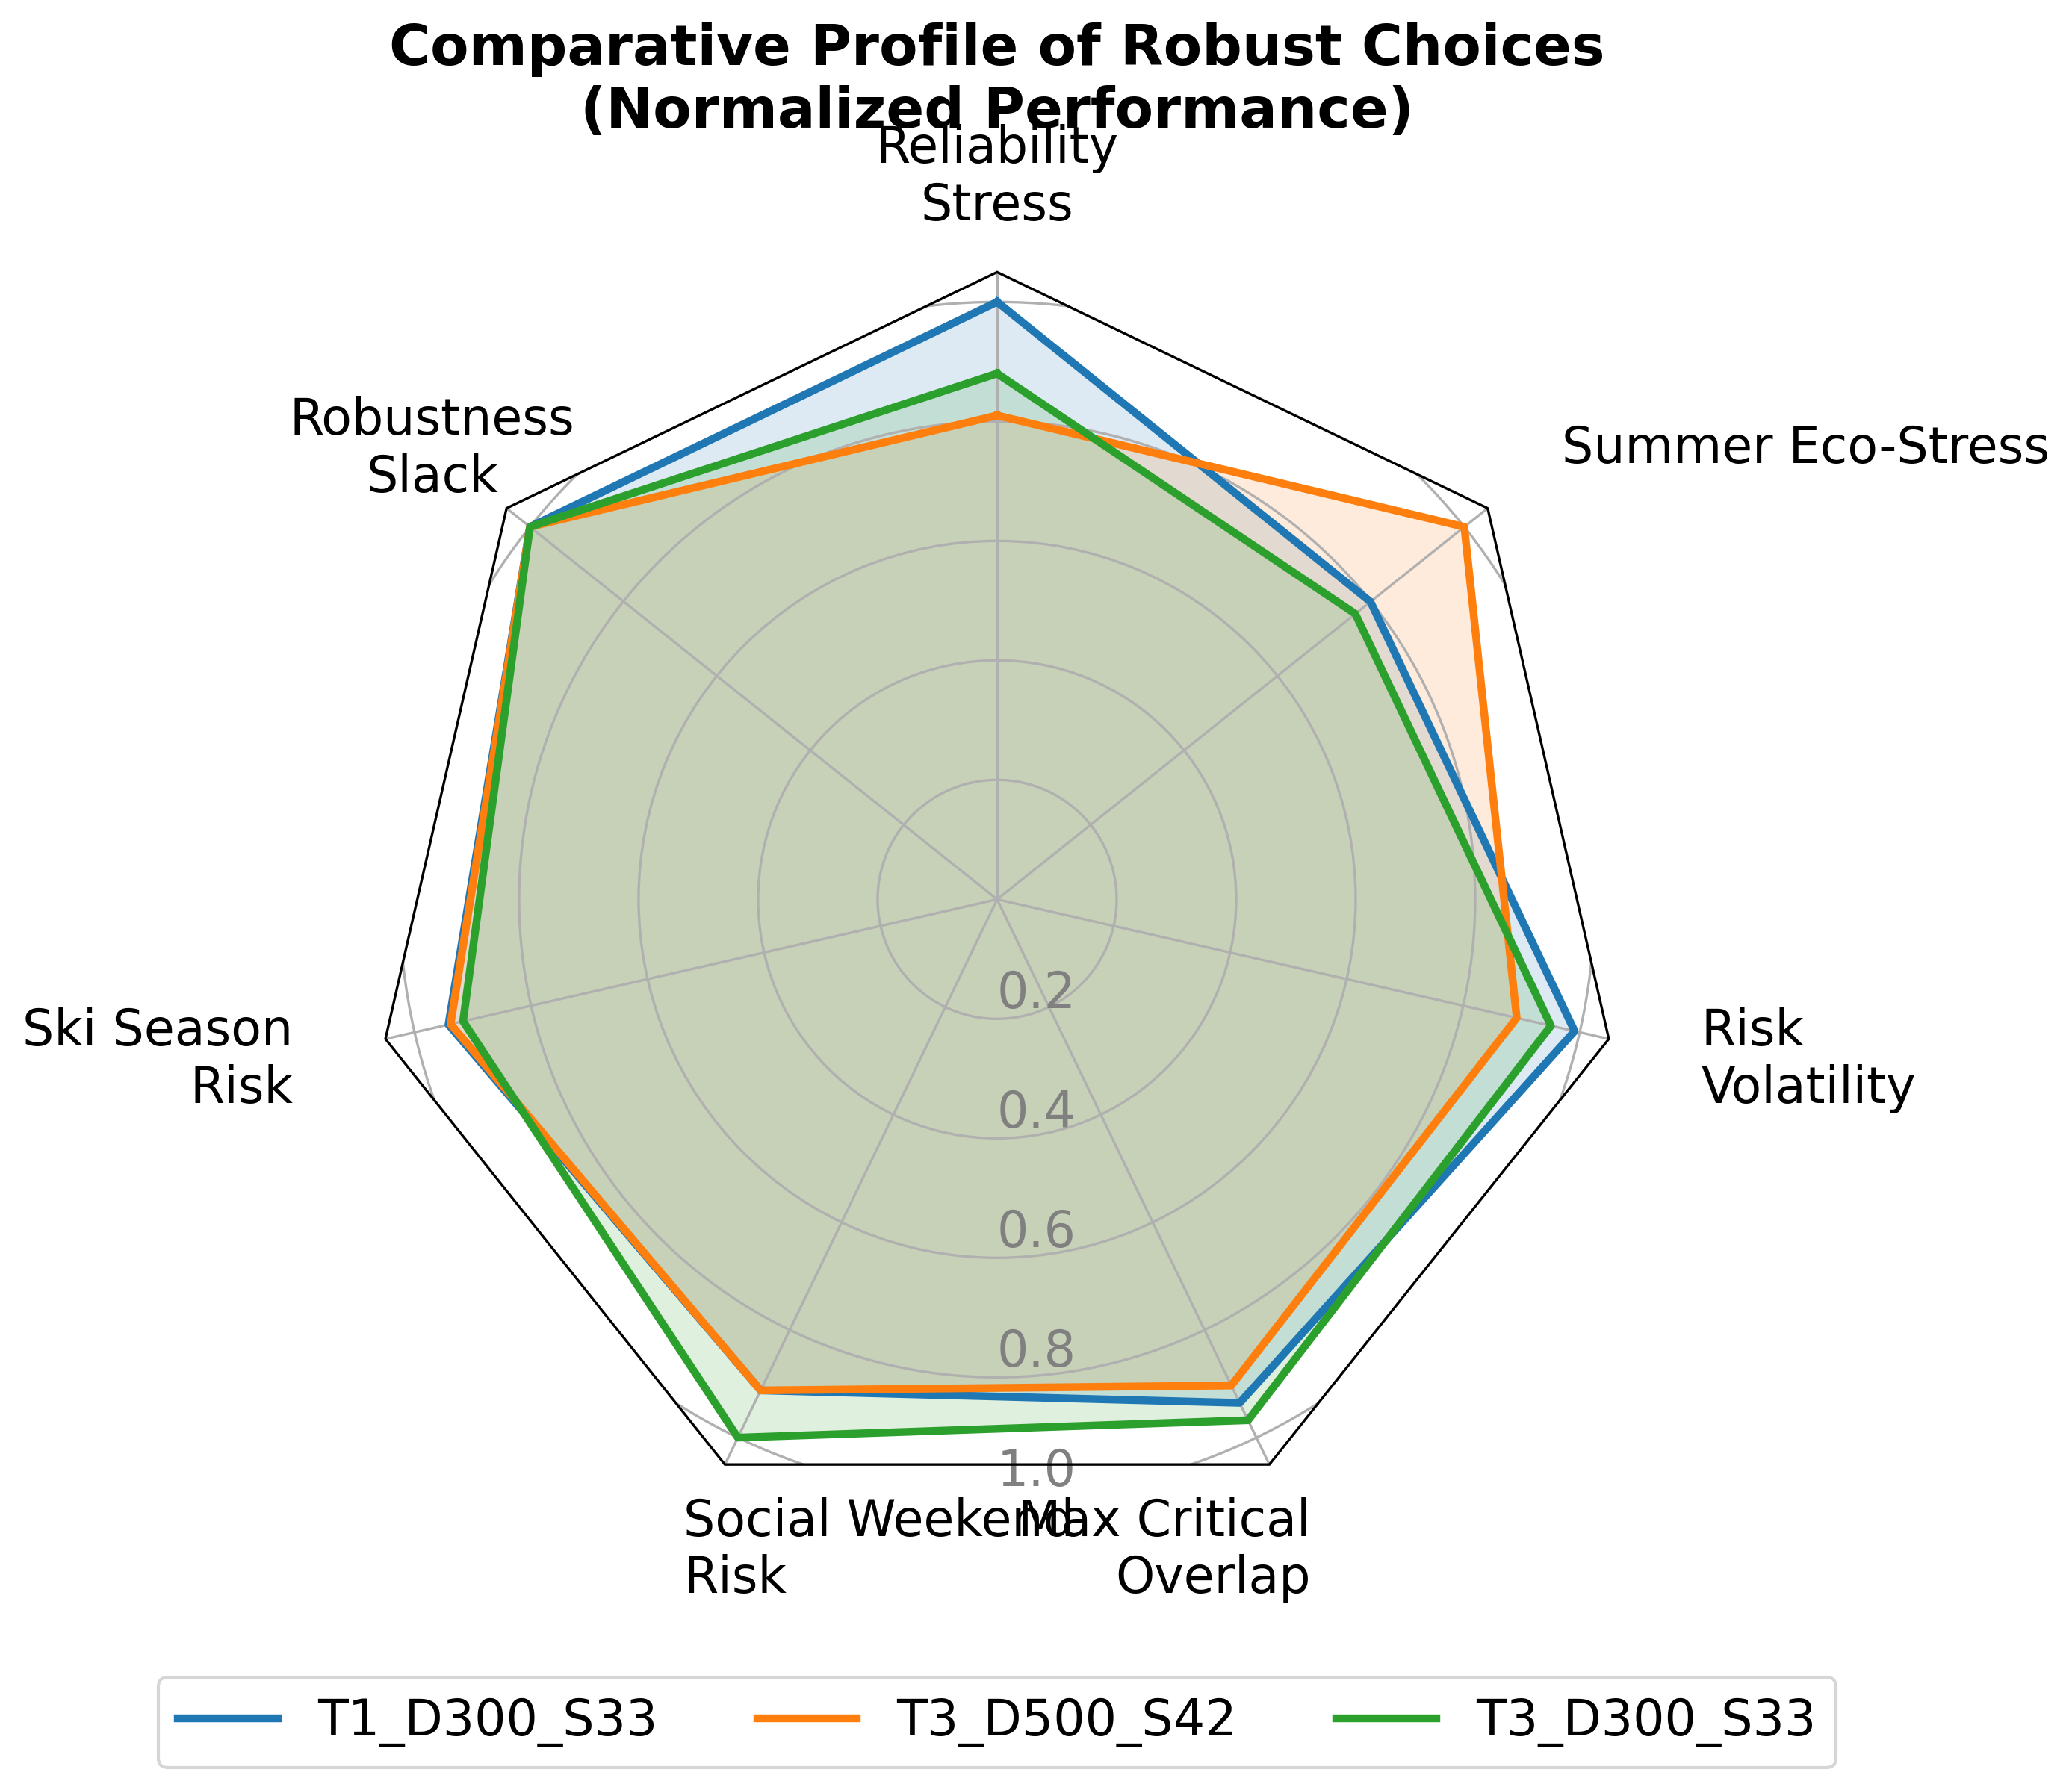
\includegraphics[width=0.7\textwidth]{figures/winners_radar_chart.png}
    \caption{Performance profiles of the three robust alternatives identified across the tested scenarios and orness intervals (normalized scale $[0,1]$). \textbf{T1\_D300\_S33} emphasizes technical reliability, \textbf{T3\_D500\_S42} combines environmental strength with operational robustness, and \textbf{T3\_D300\_S33} offers the strongest overlap and social performance within a balanced profile.}
    \label{fig:radar_chart}
\end{figure}
